\documentclass{article}
\usepackage{fancyhdr}
\usepackage[utf8]{inputenc}
\usepackage[english]{babel}
\usepackage{tikz, multicol, graphicx, etoolbox, enumerate, setspace, relsize, mathrsfs, verbatim}
\usepackage{amsmath, amsfonts, amssymb, amsthm, epsfig, epstopdf, titling, url, array, esvect, tikz-3dplot}
\usepackage{graphicx}
\usepackage{hyperref}

\usepackage{listings}
\usepackage{xcolor}

\definecolor{codegreen}{rgb}{0,0.6,0}
\definecolor{codegray}{rgb}{0.5,0.5,0.5}
\definecolor{codepurple}{rgb}{0.58,0,0.82}
\definecolor{backcolour}{rgb}{0.95,0.95,0.92}

\usepackage{pgfplots}
\usepackage{tcolorbox}
\usepackage{amsthm}
\usepackage{cancel}
\usepackage[left=1in,right=1in,top=1in,bottom=1in]{geometry}
\usepackage[tableaux]{prooftrees}

\lstdefinestyle{mystyle}{
    backgroundcolor=\color{backcolour},   
    commentstyle=\color{codegreen},
    keywordstyle=\color{magenta},
    numberstyle=\tiny\color{codegray},
    stringstyle=\color{codepurple},
    basicstyle=\ttfamily\footnotesize,
    breakatwhitespace=false,         
    breaklines=true,                 
    captionpos=b,                    
    keepspaces=true,                 
    numbers=left,                    
    numbersep=5pt,                  
    showspaces=false,                
    showstringspaces=false,
    showtabs=false,                  
    tabsize=2
}

\lstset{style=mystyle}

\pagestyle{fancy}
\fancyhf{}
\fancyhead[L,RO]{Tasksheet 5}
\fancyhead[R,RO]{Fundamentals of Computational Mathematics}
\fancyfoot[L,RO]{Xiang Gao}
\fancyfoot[R,RO]{Math 4610}
\renewcommand{\headrulewidth}{0.4pt}% Default \headrulewidth is 0.4pt
\renewcommand{\footrulewidth}{0.4pt}% Default \footrulewidth is 0pt
\def\checkmark{\tikz\fill[scale=0.4](0,.35) -- (.25,0) -- (1,.7) -- (.25,.15) -- cycle;} 

\begin{document}

\section*{Task 1}
I have created a  code that will search for the root of the given function
\begin{align}
f(x) = xe^{3x^2} - 7x
\end{align}
using Newton's method. I have also added this code to my software manual with the example results.\\
\lstinputlisting[language=Python]{Task_1.py}
This is the result I have with initial guess of $-2$, tolerable error of $0.0001$, and maximum steps of $200$ using function $(1)$:
\begin{center}
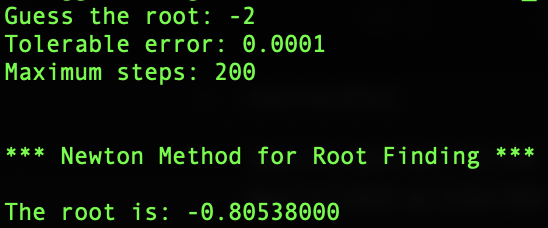
\includegraphics[width=\textwidth]{Screenshots/Newton.png}
{\bf Figure 1.} Newton's Method of Root Finding Result.
\end{center}

\newpage

\section*{Task 2}
I have repeated Task $1$ for the secant method. The code is provided below. \\
\lstinputlisting[language=Python]{Task_2.py}
This is the result I have with initial guess of $-2$, second guess of $-0.5$, tolerable error of $0.001$, and maximum steps of $200$ using function $(1)$:
\begin{center}
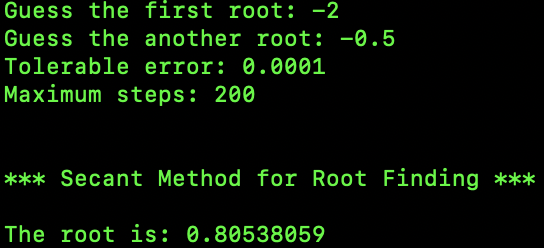
\includegraphics[width=\textwidth]{Screenshots/Secant.png}
{\bf Figure 2.} Secant Method of Root Finding Result.
\end{center}

\section*{Task 3}
As we discussed, the Newton's method is given by 
$$x_{k+1} = x_k - \dfrac{f\left(x_k\right)}{f'\left(x_k\right)}$$
In order to do a computational convergence analysis, we need to assume the real root of the function to be $x_r$. Let error be defined as the difference between each iteration and the real root. Then the error analysis would be
\begin{align*}
x_{k+1} - x_r &= x_k - \dfrac{f\left(x_k\right)}{f'\left(x_k\right)} - x_r\\
e_{k+1} & = e_k - \dfrac{f\left(x_k\right)}{f'\left(x_k\right)} \\
		& = \dfrac{e_kf'\left(x_k\right) - f\left(x_k\right)}{f'\left(x_k\right)} 
\end{align*}
Now consider the Taylor Series expansion for the error, that is
\begin{align*}
0 = f\left(x_r\right) = f\left(x_k - e_k\right) &= f\left(x_k\right) + f'\left(x_k\right)\left(x_k - x_r\right) + \dfrac{1}{2}f''(x_k)\left(x_k - x_r\right)^2+ \dots\\
& = f\left(x_k\right) + f'\left(x_k\right)\left(e_k\right) + \underbrace{\dfrac{1}{2}f''\left(\xi\right)e_k^2+ \dots}_{\text{negligible}}\\
\implies -f\left(x_k\right) - e_k f'\left(x_k\right)& = \dfrac{1}{2}f''\left(\xi\right)e_k^2
\end{align*}
Substitute this back to the previous error analysis result of $e_{k+1}$, we have
\begin{align*}
\left|e_{k+1}\right| &= \left|\dfrac{\dfrac{1}{2}f''\left(\xi\right)e_k^2}{f'\left(x_k\right)}\right|\\
				&= \underbrace{\left|\dfrac{\dfrac{1}{2}f''\left(\xi\right)}{f'\left(x_k\right)}\right|}_{\text{C}}\left|e_k^2\right|
\end{align*}
Therefore, the prior result reduces down to $\left|e_{k+1}\right|  = C \left|e_k\right|^2$, hence showing us Newton's method is quadraticly convergent. \\
Using the example from Tasksheet $4$, that is
$$f(x) = xe^{3x^2} - 7x$$
we have known at this point that one of the real root is $-0.8053$, we can make a guess of $-1$, which gives an error of 
$$e_k = \left|-0.194699999\right| \approx 0.194699999$$
Using the initial guess, $x_{k+1}$ will be
$$e_{k+1} = \left|\left(-1 - \dfrac{f(-1)}{f'(-1)}\right) -0.8053 \right|\approx 0.096753454$$
And we can see that 
$$ e_{k+1} = C e_k^2= 0.194699999^2 \approx 0.096753454$$
for $C \approx 3 $. Hence, it is suffice to say that Newton's method satisfies quadratic convergence.

\newpage

\section*{Task 4}
As we discussed, the Secant's method is given by 
$$x_{k+1} = x_k - f\left(x_k\right)\dfrac{x_k - x_{k-1}}{f\left(x_k\right) - f\left(x_{k-1}\right)}$$
In order to do a computational convergence analysis, we need to assume the real root of the function to be $x_r$. Let error be defined as the difference between each iteration and the real root. Then the error analysis would be
\begin{align*}
x_{k+1} - x_r &= x_k - f\left(x_k\right)\dfrac{x_k - x_{k-1}}{f\left(x_k\right) - f\left(x_{k-1}\right)}- x_r\\
e_{k+1} & = e_k - f\left(x_r + e_k\right)\dfrac{e_k - e_{k-1}}{f\left(x_k + e_k\right) - f\left(x_r + x_{k-1}\right)} \\
		& = e_k - \dfrac{f\left(x_r + e_k\right)\left(e_k - e_{k-1}\right)}{f\left(x_k + e_k\right) - f\left(x_r + x_{k-1}\right)}
\end{align*}
We can consider the Taylor Series expansion again for $f(x_r + e_k)$, since $f(x_r) = 0$, we have,
\begin{align*}
f(x_r + e_k) &\approx f'(x_r)e_k + \dfrac{f''(x_r)}{2}e_k^2\\
		& = e_kf'(x_r) \left(1 + \dfrac{f''(x_r)}{2f'(x_r)}e_k\right)\\
		& = e_kf'(x_r) \left(1 + Me_k\right)
\end{align*}
where $M = \dfrac{f''(x_r)}{2f'(x_r)}$ for simplicity sake. Now, we can substitute it back to the error analysis equation, and get
\begin{align*}
e_{k+1} &\approx e_k - \dfrac{e_kf'(x_r) \left(1 + Me_k\right)\left(e_k - e_{k-1}\right)}{f'(x_r)\left(e_k - e_{k-1}\right)\left(1 + M(e_k+e_{k-1})\right)}\\
		& = e_k - \dfrac{e_k\left(1 + M e_k\right)}{1 + M\left(e_k + e_{k-1}\right)}\\
		& = \dfrac{e_{k-1}e_kM}{1+ M\left(e_k + e_{k-1}\right)}\\
		&\approx e_{k-1}e_kM = \dfrac{f''(x_r)}{2f'(x_r)}e_{k-1}e_k
\end{align*}
which we can see not linear but not quadratically either as the Newton's Method. Let assume:
$$\left|e_{k-1}\right| \approx C \left|e_k\right|^p$$
Then, 
\begin{align*}
C\left|x_k\right|^p &\approx \left|M\right|\left|e_{k-1}\right|\left|e_k\right|\\
C\left|x_k\right|^{p-1} &\approx \left|M\right|\left|e_{k-1}\right|\\
\left|x_k\right|^{p-1} &\approx \dfrac{\left|M\right|}{C}\left|e_{k-1}\right|\\
\left|x_k\right| &\approx \left(\dfrac{\left|M\right|}{C}\right)^{\frac{1}{p-1}}\left|e_{k-1}\right|^{\frac{1}{p-1}}
\end{align*}
Since $p = \dfrac{1}{p-1}$, exactly how the Golden ratio is defined, that is
$$p = \dfrac{1+\sqrt{5}}{2} \approx 1.618$$
Now, we can conclude that, for the secant method, 
$$\left|e_{k+1}\right| \approx \left|\dfrac{f''(x_r)}{2f'(x_r)}\right|^{\dfrac{\sqrt{5} - 1}{2}}\left|e_k\right|^{\dfrac{\sqrt{5} - 1}{2}}$$
Checking out conclusion against the example from Tasksheet $4$, it is true.

\section*{Task 5}
The code I created for the Hybrid method is provided below.\\
\lstinputlisting[language=Python]{Task_5.py}
This is the result I have with the interval $\left[-10, -0.5\right]$, initial guess of $-5$, tolerable error of $0.0008$, and maximum steps of $80$:
\begin{center}
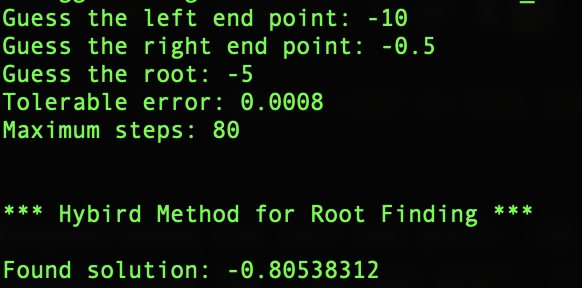
\includegraphics[width=\textwidth]{Screenshots/Hybrid.png}
{\bf Figure 3.} Hybrid Method of Root Finding Result.
\end{center}
\section*{Task 6}
From this \href{https://www.researchgate.net/publication/314387274_Comparative_Study_of_Bisection_Newton-Raphson_and_Secant_Methods_of_Root-_Finding_Problems}{journal article}\footnote{https://www.researchgate.net/publication/314387274-Comparative-Study-of-Bisection-Newton-Raphson-and-Secant-Methods-of-Root--Finding-Problems} I found, the Bisection method seems to be the slowest of the three. With the Newton and Secant methods converging to the exact root with $0.000000$ error at the $8^{th}$ and $6^{th}$ iteration respectively, the Bisection method only converges at the $52$ second iteration.\\
Even though Secant method is in general slower than the Newton's method, a factor we need to consider is the cost of convergence. That is, the Secant method only requires one function per iteration while as the Newton's method requires both the function and its derivative.
\end{document}